% Options for packages loaded elsewhere
\PassOptionsToPackage{unicode}{hyperref}
\PassOptionsToPackage{hyphens}{url}
%
\documentclass[
  a4paper,
]{article}
\usepackage{amsmath,amssymb}
\usepackage{iftex}
\ifPDFTeX
  \usepackage[T1]{fontenc}
  \usepackage[utf8]{inputenc}
  \usepackage{textcomp} % provide euro and other symbols
\else % if luatex or xetex
  \usepackage{unicode-math} % this also loads fontspec
  \defaultfontfeatures{Scale=MatchLowercase}
  \defaultfontfeatures[\rmfamily]{Ligatures=TeX,Scale=1}
\fi
\usepackage{lmodern}
\ifPDFTeX\else
  % xetex/luatex font selection
  \setmainfont[]{Helvetica}
\fi
% Use upquote if available, for straight quotes in verbatim environments
\IfFileExists{upquote.sty}{\usepackage{upquote}}{}
\IfFileExists{microtype.sty}{% use microtype if available
  \usepackage[]{microtype}
  \UseMicrotypeSet[protrusion]{basicmath} % disable protrusion for tt fonts
}{}
\makeatletter
\@ifundefined{KOMAClassName}{% if non-KOMA class
  \IfFileExists{parskip.sty}{%
    \usepackage{parskip}
  }{% else
    \setlength{\parindent}{0pt}
    \setlength{\parskip}{6pt plus 2pt minus 1pt}}
}{% if KOMA class
  \KOMAoptions{parskip=half}}
\makeatother
\usepackage{xcolor}
\usepackage[margin=0.75in]{geometry}
\usepackage{graphicx}
\makeatletter
\def\maxwidth{\ifdim\Gin@nat@width>\linewidth\linewidth\else\Gin@nat@width\fi}
\def\maxheight{\ifdim\Gin@nat@height>\textheight\textheight\else\Gin@nat@height\fi}
\makeatother
% Scale images if necessary, so that they will not overflow the page
% margins by default, and it is still possible to overwrite the defaults
% using explicit options in \includegraphics[width, height, ...]{}
\setkeys{Gin}{width=\maxwidth,height=\maxheight,keepaspectratio}
% Set default figure placement to htbp
\makeatletter
\def\fps@figure{htbp}
\makeatother
\setlength{\emergencystretch}{3em} % prevent overfull lines
\providecommand{\tightlist}{%
  \setlength{\itemsep}{0pt}\setlength{\parskip}{0pt}}
\setcounter{secnumdepth}{-\maxdimen} % remove section numbering
\usepackage{titling}
\pretitle{\begin{flushleft}}
\posttitle{\end{flushleft}}
\usepackage{booktabs}
\usepackage{longtable}
\usepackage{float}
\floatplacement{figure}{H}
\usepackage{colortbl}
\usepackage{pdflscape}
\usepackage{tabu}
\usepackage{makecell}
\usepackage{xcolor}
\usepackage{soul}
\usepackage{caption}
\usepackage[singlelinecheck=false]{caption}
\usepackage[font={small,bf}]{caption}
\usepackage{multirow}
\usepackage{array}
\usepackage{lscape}
\newcommand{\blandscape}{\begin{landscape}}
\newcommand{\elandscape}{\end{landscape}}
\usepackage[dvipsnames]{xcolor}
\renewcommand{\footnotesize}{\tiny}
\usepackage{booktabs}
\usepackage{longtable}
\usepackage{array}
\usepackage{multirow}
\usepackage{wrapfig}
\usepackage{float}
\usepackage{colortbl}
\usepackage{pdflscape}
\usepackage{tabu}
\usepackage{threeparttable}
\usepackage{threeparttablex}
\usepackage[normalem]{ulem}
\usepackage{makecell}
\usepackage{xcolor}
\ifLuaTeX
  \usepackage{selnolig}  % disable illegal ligatures
\fi
\usepackage{bookmark}
\IfFileExists{xurl.sty}{\usepackage{xurl}}{} % add URL line breaks if available
\urlstyle{same}
\hypersetup{
  hidelinks,
  pdfcreator={LaTeX via pandoc}}

\title{\vspace{-1.5cm} \begin{LARGE} WGS Quality Control Report \end{LARGE}}
\author{}
\date{\vspace{-2.5em}}

\begin{document}
\maketitle

\normalsize Batch Name: 2024-07-31

\normalsize Experiment Name: 24ARS\_NGO\_SALM\_LG73Y

\fontsize{7}{8}
\selectfont
\captionsetup[table]{labelformat=empty}
\renewcommand{\arraystretch}{1.2}

\begin{longtable}[t]{>{\centering\arraybackslash}p{1cm}>{\centering\arraybackslash}p{2cm}>{\centering\arraybackslash}p{1.5cm}>{\centering\arraybackslash}p{5.25cm}>{\centering\arraybackslash}p{5.25cm}}
\toprule
\multicolumn{1}{>{\centering\arraybackslash}p{1cm}}{\cellcolor[HTML]{D4D4D4}{\textbf{Isolate No.}}} & \multicolumn{1}{>{\centering\arraybackslash}p{2cm}}{\cellcolor[HTML]{D4D4D4}{\textbf{Sample ID}}} & \multicolumn{1}{>{\centering\arraybackslash}p{1.5cm}}{\cellcolor[HTML]{D4D4D4}{\textbf{Description}}} & \multicolumn{1}{>{\centering\arraybackslash}p{5.25cm}}{\cellcolor[HTML]{D4D4D4}{\textbf{ARSRL}}} & \multicolumn{1}{>{\centering\arraybackslash}p{5.25cm}}{\cellcolor[HTML]{D4D4D4}{\textbf{WGS}}}\\
\midrule
1 & 22ARS\_GMH0080 & NGO10 & Neisseria gonorrhoeae & Neisseria gonorrhoeae\\
\cellcolor[HTML]{FFA77F}{2} & \cellcolor[HTML]{FFA77F}{22ARS\_GMH0090} & \cellcolor[HTML]{FFA77F}{NG011} & \cellcolor[HTML]{FFA77F}{Neisseria gonorrhoeae} & \cellcolor[HTML]{FFA77F}{Neisseria gonorrhoeae}\\
3 & 22ARS\_GMH0107 & NGO12 & Neisseria gonorrhoeae & Neisseria gonorrhoeae\\
\cellcolor[HTML]{FFA77F}{4} & \cellcolor[HTML]{FFA77F}{23ARS\_GMH0023} & \cellcolor[HTML]{FFA77F}{NGO23} & \cellcolor[HTML]{FFA77F}{Klebsiella pneumoniae (x)} & \cellcolor[HTML]{FFA77F}{Neisseria gonorrhoeae}\\
\cellcolor[HTML]{FFA77F}{5} & \cellcolor[HTML]{FFA77F}{23ARS\_MAR0190} & \cellcolor[HTML]{FFA77F}{NGO25} & \cellcolor[HTML]{FFA77F}{Neisseria gonorrhoeae} & \cellcolor[HTML]{FFA77F}{Neisseria gonorrhoeae}\\
\addlinespace
6 & 23ARS\_MAR0191 & NGO26 & Neisseria gonorrhoeae & Neisseria gonorrhoeae\\
\cellcolor[HTML]{FFA77F}{7} & \cellcolor[HTML]{FFA77F}{23ARS\_MAR0247} & \cellcolor[HTML]{FFA77F}{NGO27} & \cellcolor[HTML]{FFA77F}{Neisseria gonorrhoeae} & \cellcolor[HTML]{FFA77F}{Neisseria gonorrhoeae}\\
8 & 23ARS\_RTH0001 & NGO28 & Neisseria gonorrhoeae & Neisseria gonorrhoeae\\
9 & 23ARS\_RTH0003 & NGO30 & Neisseria gonorrhoeae & Neisseria gonorrhoeae\\
10 & 23ARS\_RTH0004 & NGO31 & Neisseria gonorrhoeae & Neisseria gonorrhoeae\\
\addlinespace
11 & 23ARS\_RTH0005 & NGO32 & Neisseria gonorrhoeae & Neisseria gonorrhoeae\\
\cellcolor[HTML]{FFA77F}{12} & \cellcolor[HTML]{FFA77F}{23ARS\_SLH0024} & \cellcolor[HTML]{FFA77F}{NGO33} & \cellcolor[HTML]{FFA77F}{Neisseria gonorrhoeae} & \cellcolor[HTML]{FFA77F}{Neisseria gonorrhoeae}\\
13 & 23ARS\_SLH0025 & NGO34 & Neisseria gonorrhoeae & Neisseria gonorrhoeae\\
14 & 23ARS\_SLH0026 & NGO35 & Neisseria gonorrhoeae & Neisseria gonorrhoeae\\
15 & 23ARS\_VSM0001 & NGO36 & Neisseria gonorrhoeae & Neisseria gonorrhoeae\\
\addlinespace
16 & 23ARS\_VSM0033 & NGO37 & Neisseria gonorrhoeae & Neisseria gonorrhoeae\\
17 & 23ARS\_VSM0098 & NGO38 & Neisseria gonorrhoeae & Neisseria gonorrhoeae\\
18 & 23ARS\_VSM0181 & NGO41 & Neisseria gonorrhoeae & Neisseria gonorrhoeae\\
19 & 23ARS\_VSM0477 & NGO44 & Neisseria gonorrhoeae & Neisseria gonorrhoeae\\
20 & 23ARS\_VSM0600 & NGO45 & Neisseria gonorrhoeae & Neisseria gonorrhoeae\\
\addlinespace
\cellcolor[HTML]{FFA77F}{21} & \cellcolor[HTML]{FFA77F}{24ARS\_BRH0016} & \cellcolor[HTML]{FFA77F}{NGO47} & \cellcolor[HTML]{FFA77F}{*Neisseria gonorrhoeae} & \cellcolor[HTML]{FFA77F}{Neisseria gonorrhoeae}\\
\cellcolor[HTML]{FFA77F}{22} & \cellcolor[HTML]{FFA77F}{24ARS\_CVM0067} & \cellcolor[HTML]{FFA77F}{NGO49} & \cellcolor[HTML]{FFA77F}{Neisseria gonorrhoeae} & \cellcolor[HTML]{FFA77F}{Neisseria gonorrhoeae}\\
\bottomrule
\multicolumn{5}{l}{\rule{0pt}{1em}\textit{Legend:} PASS   |   \colorbox{Peach}{WARNING}   |   \colorbox{Salmon}{FAILURE}   |   \textcolor{Blue}{EXCEEDS THRESHOLD METRIC/S}   |   (x) - NON-CONCORDANT   |}\\
\end{longtable}

\fontsize{7}{8}
\selectfont
\captionsetup[table]{labelformat=empty}
\renewcommand{\arraystretch}{1.2}

\(\\\)

\fontsize{7}{8}
\selectfont
\captionsetup[table]{labelformat=empty}
\renewcommand{\arraystretch}{1.2}

\begin{ThreePartTable}
\begin{TableNotes}[para]
\item \textit{Legend:} 
\item PASS
\item   |  
\item \colorbox{Peach}{WARNING}
\item   |  
\item \colorbox{Salmon}{FAILURE}
\item   |  
\item \textcolor{Blue}{EXCEEDS THRESHOLD METRIC/S}
\item   |  
\end{TableNotes}
\begin{longtable}[t]{>{\centering\arraybackslash}p{1cm}>{\centering\arraybackslash}p{3cm}>{\centering\arraybackslash}p{2cm}>{\centering\arraybackslash}p{2cm}>{\centering\arraybackslash}p{2cm}>{\centering\arraybackslash}p{2cm}>{\centering\arraybackslash}p{2cm}}
\toprule
\multicolumn{1}{>{\centering\arraybackslash}p{1cm}}{\cellcolor[HTML]{D4D4D4}{\textbf{Isolate No.}}} & \multicolumn{1}{>{\centering\arraybackslash}p{3cm}}{\cellcolor[HTML]{D4D4D4}{\textbf{Sample ID}}} & \multicolumn{1}{>{\centering\arraybackslash}p{2cm}}{\cellcolor[HTML]{D4D4D4}{\textbf{Contamination}}} & \multicolumn{1}{>{\centering\arraybackslash}p{2cm}}{\cellcolor[HTML]{D4D4D4}{\textbf{Contigs}}} & \multicolumn{1}{>{\centering\arraybackslash}p{2cm}}{\cellcolor[HTML]{D4D4D4}{\textbf{GC Percent}}} & \multicolumn{1}{>{\centering\arraybackslash}p{2cm}}{\cellcolor[HTML]{D4D4D4}{\textbf{N50}}} & \multicolumn{1}{>{\centering\arraybackslash}p{2cm}}{\cellcolor[HTML]{D4D4D4}{\textbf{Total Length}}}\\
\midrule
1 & 22ARS\_GMH0080 & \textcolor{black}{0} & \textcolor{black}{103} & 52.50 & \textcolor{black}{51133} & 2116760\\
\cellcolor[HTML]{FFA77F}{2} & \cellcolor[HTML]{FFA77F}{22ARS\_GMH0090} & \cellcolor[HTML]{FFA77F}{\textcolor{black}{0}} & \cellcolor[HTML]{FFA77F}{\textcolor{black}{334}} & \cellcolor[HTML]{FFA77F}{52.58} & \cellcolor[HTML]{FFA77F}{\textcolor{blue}{47270}} & \cellcolor[HTML]{FFA77F}{2140550}\\
3 & 22ARS\_GMH0107 & \textcolor{black}{0} & \textcolor{black}{84} & 52.59 & \textcolor{black}{66604} & 2112654\\
\cellcolor[HTML]{FFA77F}{4} & \cellcolor[HTML]{FFA77F}{23ARS\_GMH0023} & \cellcolor[HTML]{FFA77F}{\textcolor{black}{0}} & \cellcolor[HTML]{FFA77F}{\textcolor{black}{93}} & \cellcolor[HTML]{FFA77F}{52.51} & \cellcolor[HTML]{FFA77F}{\textcolor{blue}{48995}} & \cellcolor[HTML]{FFA77F}{2122470}\\
\cellcolor[HTML]{FFA77F}{5} & \cellcolor[HTML]{FFA77F}{23ARS\_MAR0190} & \cellcolor[HTML]{FFA77F}{\textcolor{black}{0}} & \cellcolor[HTML]{FFA77F}{\textcolor{black}{246}} & \cellcolor[HTML]{FFA77F}{53.11} & \cellcolor[HTML]{FFA77F}{\textcolor{black}{52455}} & \cellcolor[HTML]{FFA77F}{2126635}\\
\addlinespace
6 & 23ARS\_MAR0191 & \textcolor{black}{0} & \textcolor{black}{91} & 52.46 & \textcolor{black}{50579} & 2125474\\
\cellcolor[HTML]{FFA77F}{7} & \cellcolor[HTML]{FFA77F}{23ARS\_MAR0247} & \cellcolor[HTML]{FFA77F}{\textcolor{black}{0}} & \cellcolor[HTML]{FFA77F}{\textcolor{black}{94}} & \cellcolor[HTML]{FFA77F}{52.52} & \cellcolor[HTML]{FFA77F}{\textcolor{blue}{48929}} & \cellcolor[HTML]{FFA77F}{2110602}\\
8 & 23ARS\_RTH0001 & \textcolor{black}{0} & \textcolor{black}{96} & 52.30 & \textcolor{black}{59062} & 2176872\\
9 & 23ARS\_RTH0003 & \textcolor{black}{0} & \textcolor{black}{91} & 52.39 & \textcolor{black}{60238} & 2129311\\
10 & 23ARS\_RTH0004 & \textcolor{black}{0} & \textcolor{black}{93} & 52.57 & \textcolor{black}{51395} & 2108718\\
\addlinespace
11 & 23ARS\_RTH0005 & \textcolor{black}{0} & \textcolor{black}{90} & 52.61 & \textcolor{black}{58813} & 2074248\\
\cellcolor[HTML]{FFA77F}{12} & \cellcolor[HTML]{FFA77F}{23ARS\_SLH0024} & \cellcolor[HTML]{FFA77F}{\textcolor{black}{0}} & \cellcolor[HTML]{FFA77F}{\textcolor{black}{92}} & \cellcolor[HTML]{FFA77F}{52.51} & \cellcolor[HTML]{FFA77F}{\textcolor{blue}{47038}} & \cellcolor[HTML]{FFA77F}{2123959}\\
13 & 23ARS\_SLH0025 & \textcolor{black}{0} & \textcolor{black}{84} & 52.65 & \textcolor{black}{59337} & 2072515\\
14 & 23ARS\_SLH0026 & \textcolor{black}{0} & \textcolor{black}{103} & 52.30 & \textcolor{black}{58032} & 2178857\\
15 & 23ARS\_VSM0001 & \textcolor{black}{0} & \textcolor{black}{94} & 52.53 & \textcolor{black}{57227} & 2110956\\
\addlinespace
16 & 23ARS\_VSM0033 & \textcolor{black}{0} & \textcolor{black}{84} & 52.51 & \textcolor{black}{51589} & 2123578\\
17 & 23ARS\_VSM0098 & \textcolor{black}{0} & \textcolor{black}{83} & 52.55 & \textcolor{black}{56625} & 2118400\\
18 & 23ARS\_VSM0181 & \textcolor{black}{0} & \textcolor{black}{102} & 52.50 & \textcolor{black}{52615} & 2124581\\
19 & 23ARS\_VSM0477 & \textcolor{black}{0} & \textcolor{black}{94} & 52.50 & \textcolor{black}{58791} & 2120954\\
20 & 23ARS\_VSM0600 & \textcolor{black}{0} & \textcolor{black}{93} & 52.40 & \textcolor{black}{50730} & 2133253\\
\addlinespace
\cellcolor[HTML]{FFA77F}{21} & \cellcolor[HTML]{FFA77F}{24ARS\_BRH0016} & \cellcolor[HTML]{FFA77F}{\textcolor{black}{0}} & \cellcolor[HTML]{FFA77F}{\textcolor{black}{92}} & \cellcolor[HTML]{FFA77F}{52.49} & \cellcolor[HTML]{FFA77F}{\textcolor{blue}{49138}} & \cellcolor[HTML]{FFA77F}{2121615}\\
\cellcolor[HTML]{FFA77F}{22} & \cellcolor[HTML]{FFA77F}{24ARS\_CVM0067} & \cellcolor[HTML]{FFA77F}{\textcolor{black}{0}} & \cellcolor[HTML]{FFA77F}{\textcolor{black}{94}} & \cellcolor[HTML]{FFA77F}{52.50} & \cellcolor[HTML]{FFA77F}{\textcolor{blue}{49068}} & \cellcolor[HTML]{FFA77F}{2126365}\\
\bottomrule
\multicolumn{7}{l}{\rule{0pt}{1em}\textit{Note: } *Isolates were tagged with warning due to uncertain results  of species identification using bactinspector or sequence identification levels.}\\
\insertTableNotes
\end{longtable}
\end{ThreePartTable}

\fontsize{7}{8}
\selectfont
\captionsetup[table]{labelformat=empty}
\renewcommand{\arraystretch}{1.2}

\begin{longtable}[t]{>{\centering\arraybackslash}p{2cm}>{\raggedright\arraybackslash}p{3cm}>{\centering\arraybackslash}p{11cm}}
\toprule
\multicolumn{3}{l}{\textbf{With Warning/s}} \\
\cmidrule(l{3pt}r{3pt}){1-3}
\multicolumn{1}{>{\centering\arraybackslash}p{2cm}}{\cellcolor[HTML]{D4D4D4}{\textbf{Isolate No.}}} & \multicolumn{1}{>{\centering\arraybackslash}p{3cm}}{\cellcolor[HTML]{D4D4D4}{\textbf{Sample ID}}} & \multicolumn{1}{>{\centering\arraybackslash}p{11cm}}{\cellcolor[HTML]{D4D4D4}{\textbf{Value with warning/s}}}\\
\midrule
\cellcolor{gray!10}{2} & \cellcolor{gray!10}{22ARS\_GMH0090} & \cellcolor{gray!10}{fastqc.1.Per.sequence.GC.content.metric\_value, fastqc.1.Sequence.Duplication.Levels.metric\_value, fastqc.1.Sequence.Length.Distribution.metric\_value, fastqc.2.Per.sequence.GC.content.metric\_value, fastqc.2.Sequence.Duplication.Levels.metric\_value, fastqc.2.Sequence.Length.Distribution.metric\_value}\\
4 & 23ARS\_GMH0023 & fastqc.1.Per.sequence.GC.content.metric\_value, fastqc.1.Sequence.Duplication.Levels.metric\_value, fastqc.1.Sequence.Length.Distribution.metric\_value, fastqc.2.Per.sequence.GC.content.metric\_value, fastqc.2.Sequence.Duplication.Levels.metric\_value, fastqc.2.Sequence.Length.Distribution.metric\_value\\
\cellcolor{gray!10}{5} & \cellcolor{gray!10}{23ARS\_MAR0190} & \cellcolor{gray!10}{fastqc.1.Per.sequence.GC.content.metric\_value, fastqc.1.Sequence.Duplication.Levels.metric\_value, fastqc.1.Sequence.Length.Distribution.metric\_value, fastqc.2.Per.sequence.GC.content.metric\_value, fastqc.2.Sequence.Duplication.Levels.metric\_value, fastqc.2.Sequence.Length.Distribution.metric\_value}\\
7 & 23ARS\_MAR0247 & fastqc.1.Per.sequence.GC.content.metric\_value, fastqc.1.Sequence.Duplication.Levels.metric\_value, fastqc.1.Sequence.Length.Distribution.metric\_value, fastqc.2.Per.sequence.GC.content.metric\_value, fastqc.2.Sequence.Duplication.Levels.metric\_value, fastqc.2.Sequence.Length.Distribution.metric\_value\\
\cellcolor{gray!10}{12} & \cellcolor{gray!10}{23ARS\_SLH0024} & \cellcolor{gray!10}{fastqc.1.Per.sequence.GC.content.metric\_value, fastqc.1.Sequence.Duplication.Levels.metric\_value, fastqc.1.Sequence.Length.Distribution.metric\_value, fastqc.2.Per.sequence.GC.content.metric\_value, fastqc.2.Sequence.Duplication.Levels.metric\_value, fastqc.2.Sequence.Length.Distribution.metric\_value}\\
\addlinespace
21 & 24ARS\_BRH0016 & fastqc.1.Per.sequence.GC.content.metric\_value, fastqc.1.Sequence.Duplication.Levels.metric\_value, fastqc.1.Sequence.Length.Distribution.metric\_value, fastqc.2.Per.sequence.GC.content.metric\_value, fastqc.2.Sequence.Duplication.Levels.metric\_value, fastqc.2.Sequence.Length.Distribution.metric\_value\\
\cellcolor{gray!10}{22} & \cellcolor{gray!10}{24ARS\_CVM0067} & \cellcolor{gray!10}{fastqc.1.Per.sequence.GC.content.metric\_value, fastqc.1.Sequence.Duplication.Levels.metric\_value, fastqc.1.Sequence.Length.Distribution.metric\_value, fastqc.2.Per.sequence.GC.content.metric\_value, fastqc.2.Sequence.Duplication.Levels.metric\_value, fastqc.2.Sequence.Length.Distribution.metric\_value}\\
\bottomrule
\end{longtable}

\begin{longtable}[l]{>{\centering\arraybackslash}p{3cm}>{\centering\arraybackslash}p{12cm}}
\toprule
\multicolumn{2}{l}{\textbf{List of samples above/below QC threshold metrics}} \\
\cmidrule(l{3pt}r{3pt}){1-2}
\cellcolor[HTML]{D4D4D4}{\textbf{Sample ID}} & \cellcolor[HTML]{D4D4D4}{\textbf{Remarks}}\\
\midrule
 & No QC failures found.\\
\bottomrule
\end{longtable}

\fontsize{7}{8}
\selectfont
\captionsetup[table]{labelformat=empty}
\renewcommand{\arraystretch}{1.2}

\begin{longtable}[l]{>{\raggedright\arraybackslash}p{8cm}c}
\toprule
\cellcolor[HTML]{D4D4D4}{\textbf{WGS\_ID}} & \cellcolor[HTML]{D4D4D4}{\textbf{Number}}\\
\midrule
Neisseria gonorrhoeae & 22\\
\bottomrule
\end{longtable}

\begin{itemize}
\item
  \(\color{red}1\) distinct species were identified among
  \(\color{red}22\) isolates.
\item
  \(\color{red}68.18\) \% (n=15) of the isolates passed the QC, while
  \(\color{red}31.82\) \% (n=7) were tagged with warning.
\item
  Concordance between ARSRL and WGS species report was
  \(\color{red}95.45\) \%. \(\\\)
\end{itemize}

\subsubsection{GRAPHS}\label{graphs}

\fontsize{7}{8}
\selectfont
\captionsetup[table]{labelformat=empty}
\renewcommand{\arraystretch}{1.2}

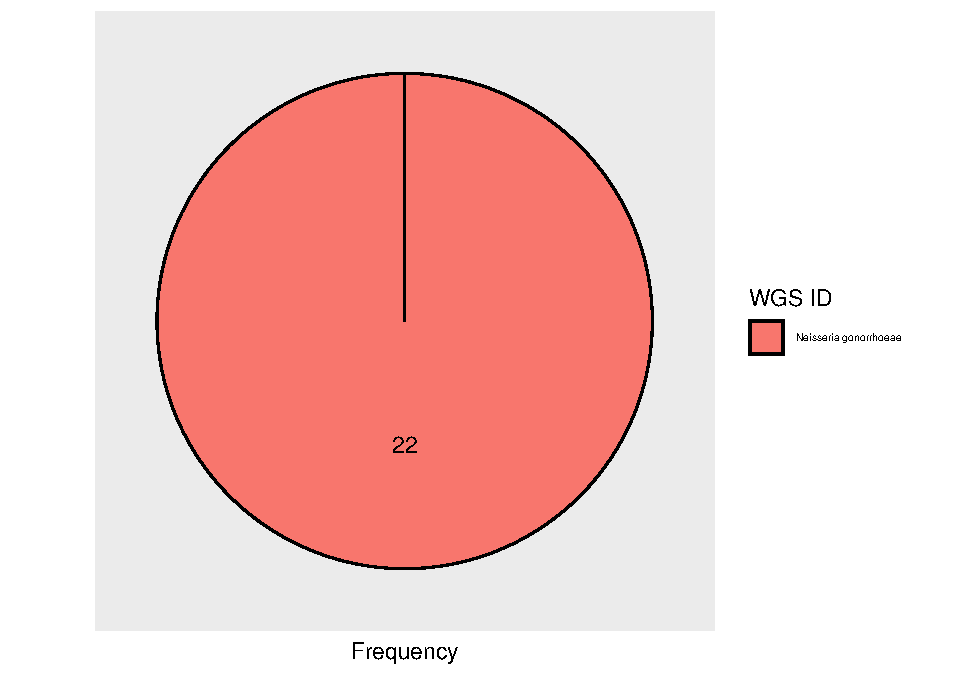
\includegraphics{qualifyr_report_2024-07-31_files/figure-latex/pie_chart-1.pdf}

\subsubsection{Result Classification}\label{result-classification}

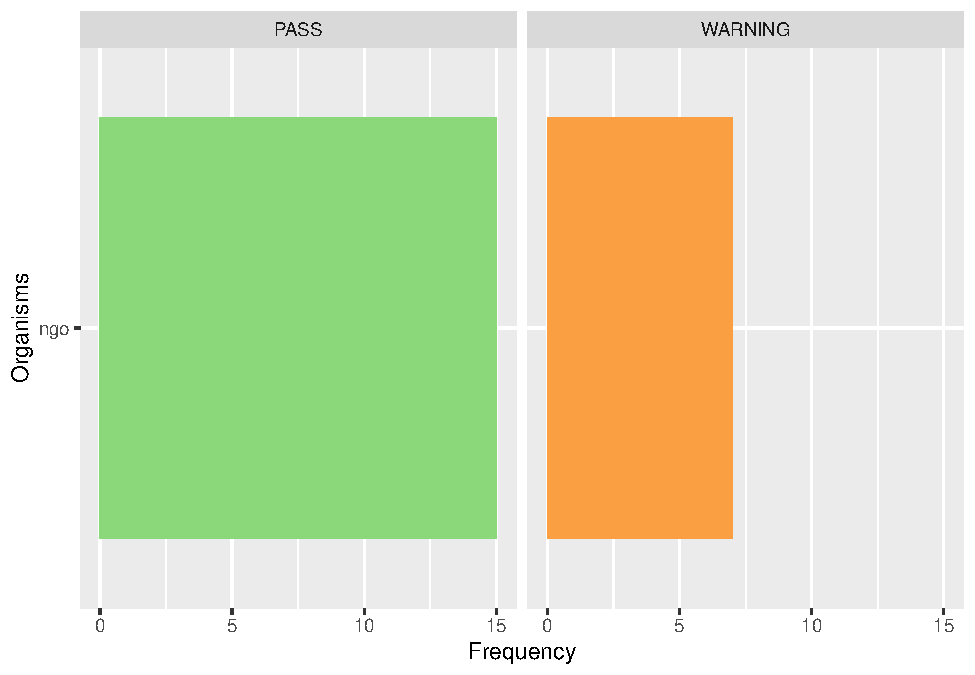
\includegraphics{qualifyr_report_2024-07-31_files/figure-latex/organism results-1.pdf}

\subsubsection{Number of contigs}\label{number-of-contigs}

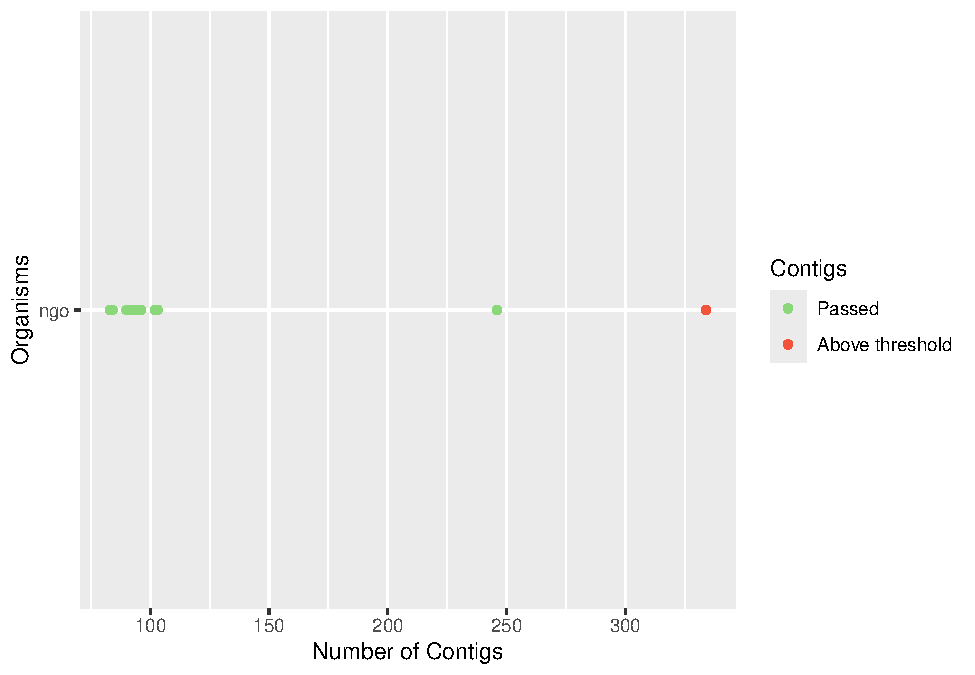
\includegraphics{qualifyr_report_2024-07-31_files/figure-latex/unnamed-chunk-1-1.pdf}

\subsubsection{N50 Value}\label{n50-value}

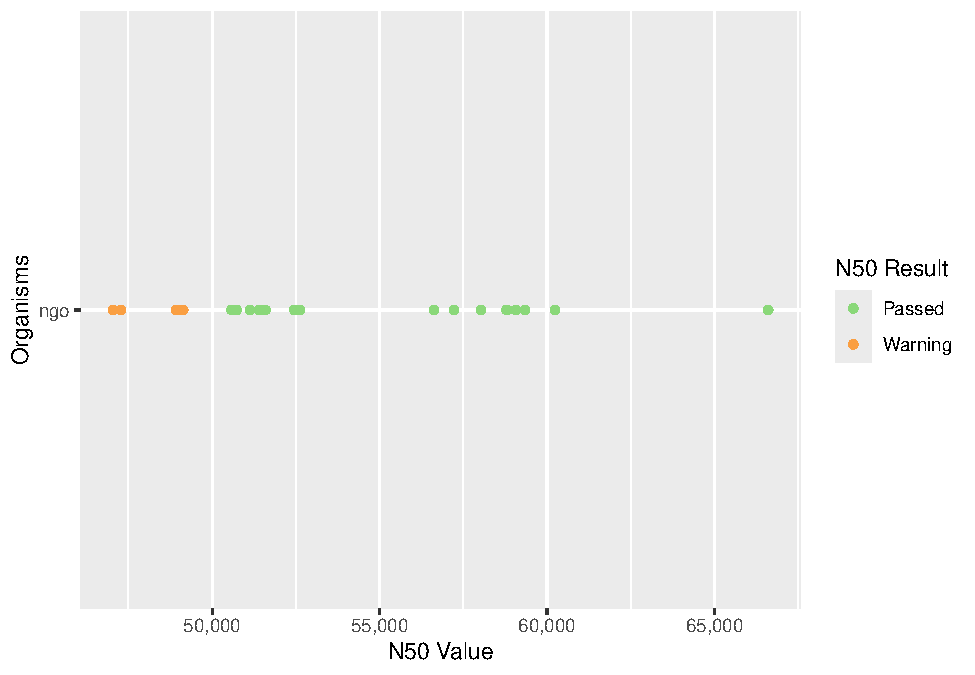
\includegraphics{qualifyr_report_2024-07-31_files/figure-latex/n50_result -1.pdf}

\subsubsection{Total Length}\label{total-length}

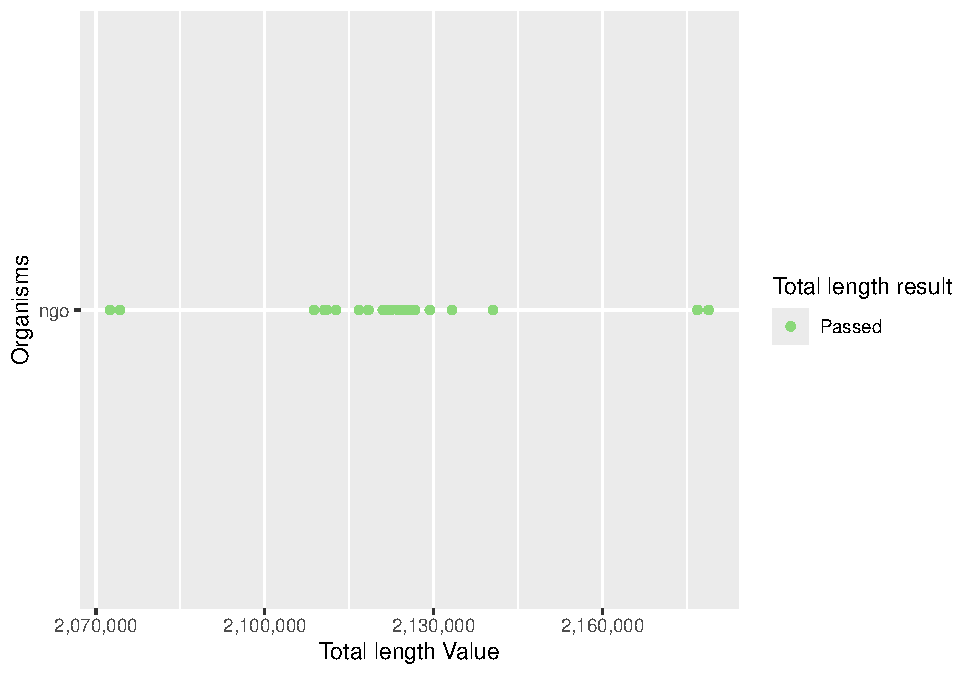
\includegraphics{qualifyr_report_2024-07-31_files/figure-latex/length_result -1.pdf}

\(\\\)

\subsubsection{RECOMMENDATION:}\label{recommendation}

\begin{longtable}[l]{>{\centering\arraybackslash}p{6cm}>{\centering\arraybackslash}p{4cm}>{\centering\arraybackslash}p{6cm}}
\toprule
\cellcolor[HTML]{D4D4D4}{\textbf{Sample ID}} & \cellcolor[HTML]{D4D4D4}{\textbf{Action}} & \cellcolor[HTML]{D4D4D4}{\textbf{Reason}}\\
\midrule
No futher action required for this batch &  & \\
\bottomrule
\end{longtable}

\subsubsection{MLST RESULTS}\label{mlst-results}

\begin{longtable}[l]{>{\centering\arraybackslash}p{3cm}>{\centering\arraybackslash}p{3cm}>{\centering\arraybackslash}p{1cm}>{\centering\arraybackslash}p{1cm}>{\centering\arraybackslash}p{1cm}>{\centering\arraybackslash}p{1cm}>{\centering\arraybackslash}p{1cm}>{\centering\arraybackslash}p{1cm}>{\centering\arraybackslash}p{1cm}c}
\toprule
\cellcolor[HTML]{D4D4D4}{\textbf{sample\_id}} & \cellcolor[HTML]{D4D4D4}{\textbf{species}} & \cellcolor[HTML]{D4D4D4}{\textbf{MLST}} & \cellcolor[HTML]{D4D4D4}{\textbf{abcZ.59.}} & \cellcolor[HTML]{D4D4D4}{\textbf{adk}} & \cellcolor[HTML]{D4D4D4}{\textbf{aroE}} & \cellcolor[HTML]{D4D4D4}{\textbf{fumC}} & \cellcolor[HTML]{D4D4D4}{\textbf{gdh}} & \cellcolor[HTML]{D4D4D4}{\textbf{pdhC}} & \cellcolor[HTML]{D4D4D4}{\textbf{pgm}}\\
\midrule
22ARS\_GMH0080 & Neisseria gonorrhoeae & 7363 & abcZ(59) & 39 & 67 & 78 & 148 & 153 & 65\\
22ARS\_GMH0090 & Neisseria gonorrhoeae & 1583 & abcZ(59) & 39 & 67 & 111 & 148 & 153 & 65\\
22ARS\_GMH0107 & Neisseria gonorrhoeae & 1582 & abcZ(59) & 39 & 170 & 78 & 148 & 154 & 65\\
23ARS\_GMH0023 & Neisseria gonorrhoeae & 7363 & abcZ(59) & 39 & 67 & 78 & 148 & 153 & 65\\
23ARS\_MAR0190 & Neisseria gonorrhoeae & 7363 & abcZ(59) & 39 & 67 & 78 & 148 & 153 & 65\\
\addlinespace
23ARS\_MAR0191 & Neisseria gonorrhoeae & 11249 & abcZ(59) & 39 & 67 & 157 & 148 & 71 & 65\\
23ARS\_MAR0247 & Neisseria gonorrhoeae & 10316 & abcZ(59) & 39 & 67 & 157 & 149 & 71 & 65\\
23ARS\_RTH0001 & Neisseria gonorrhoeae & 7827 & abcZ(59) & 39 & 67 & 158 & 148 & 153 & 65\\
23ARS\_RTH0003 & Neisseria gonorrhoeae & 14312 & abcZ(59) & 39 & 170 & 157 & 148 & 71 & 133\\
23ARS\_RTH0004 & Neisseria gonorrhoeae & 8130 & abcZ(59) & 39 & 170 & 78 & 149 & 154 & 65\\
\addlinespace
23ARS\_SLH0024 & Neisseria gonorrhoeae & 17546 & abcZ(435) & 39 & 170 & 111 & 148 & 71 & 65\\
23ARS\_SLH0025 & Neisseria gonorrhoeae & - & abcZ(59) & 39 & 67 & 158 & 149 & 71 & \textasciitilde{}65\\
23ARS\_SLH0026 & Neisseria gonorrhoeae & 7823 & abcZ(435) & 39 & 170 & 111 & 148 & 153 & 65\\
23ARS\_VSM0001 & Neisseria gonorrhoeae & 8130 & abcZ(59) & 39 & 170 & 78 & 149 & 154 & 65\\
23ARS\_VSM0033 & Neisseria gonorrhoeae & 1587 & abcZ(59) & 39 & 67 & 78 & 148 & 153 & 133\\
\addlinespace
23ARS\_VSM0098 & Neisseria gonorrhoeae & 12982 & abcZ(59) & 39 & 67 & 158 & 148 & 71 & 133\\
23ARS\_VSM0181 & Neisseria gonorrhoeae & 7363 & abcZ(59) & 39 & 67 & 78 & 148 & 153 & 65\\
23ARS\_VSM0477 & Neisseria gonorrhoeae & 7356 & abcZ(109) & 39 & 67 & 78 & 148 & 153 & 65\\
23ARS\_VSM0600 & Neisseria gonorrhoeae & 8776 & abcZ(59) & 39 & 67 & 157 & 148 & 71 & 133\\
24ARS\_BRH0016 & Neisseria gonorrhoeae & 14105 & abcZ(59) & 142 & 67 & 78 & 149 & 153 & 133\\
\addlinespace
24ARS\_CVM0067 & Neisseria gonorrhoeae & 7363 & abcZ(59) & 39 & 67 & 78 & 148 & 153 & 65\\
\bottomrule
\multicolumn{10}{l}{\rule{0pt}{1em}\textit{Legend: } (-) Not identified}\\
\end{longtable}

\subsubsection{MLST RESULTS SUMMARY:}\label{mlst-results-summary}

\begin{longtable}[l]{>{\raggedright\arraybackslash}p{6cm}>{\raggedright\arraybackslash}p{10cm}}
\toprule
\cellcolor[HTML]{D4D4D4}{\textbf{wgs\_id}} & \cellcolor[HTML]{D4D4D4}{\textbf{mlst\_count}}\\
\midrule
Neisseria gonorrhoeae & - (n= 1 ), 10316 (n= 1 ), 11249 (n= 1 ), 12982 (n= 1 ), 14105 (n= 1 ), 14312 (n= 1 ), 1582 (n= 1 ), 1583 (n= 1 ), 1587 (n= 1 ), 17546 (n= 1 ), 7356 (n= 1 ), 7363 (n= 5 ), 7823 (n= 1 ), 7827 (n= 1 ), 8130 (n= 2 ), 8776 (n= 1 )\\
\bottomrule
\multicolumn{2}{l}{\rule{0pt}{1em}\textit{Legend: } (-) Not identified}\\
\end{longtable}

\newpage
\begin{landscape}
\fontsize{7}{8}
\selectfont
\captionsetup[table]{labelformat=empty}
\renewcommand{\arraystretch}{1.2}

\subsubsection{AMR PREDICTION RESULTS}\label{amr-prediction-results}

\begin{tabular}{c>{\centering\arraybackslash}p{3cm}>{\centering\arraybackslash}p{3cm}>{\centering\arraybackslash}p{3cm}>{\centering\arraybackslash}p{3cm}}
\toprule
\multicolumn{5}{l}{\textbf{\textit{Neisseria gonorrhoeae}}} \\
\cmidrule(l{3pt}r{3pt}){1-5}
\cellcolor[HTML]{D4D4D4}{\textbf{sample\_id}} & \cellcolor[HTML]{D4D4D4}{\textbf{AMR BETA-LACTAM}} & \cellcolor[HTML]{D4D4D4}{\textbf{AMR EFFLUX}} & \cellcolor[HTML]{D4D4D4}{\textbf{AMR TETRACYCLINE}} & \cellcolor[HTML]{D4D4D4}{\textbf{STRESS EFFLUX}}\\
\midrule
22ARS\_GMH0080 & blaTEM-1 & norM, mtrC, mtrR, mtrA, farB & tet(M) & mtrF\\
22ARS\_GMH0090 & blaTEM-1 & mtrC, mtrR, norM, mtrA, farB & tet(M) & mtrF\\
22ARS\_GMH0107 & blaTEM-135 & norM, mtrC, mtrR, mtrA, farB & NA & mtrF\\
23ARS\_GMH0023 & blaTEM-1 & mtrC, mtrR, farB, norM, mtrA & tet(M) & mtrF\\
23ARS\_MAR0190 & blaTEM-1 & norM, mtrC, mtrR, mtrA, farB & tet(M) & mtrF\\
\addlinespace
23ARS\_MAR0191 & blaTEM-1 & mtrC, mtrR, norM, mtrA, farB & NA & mtrF\\
23ARS\_MAR0247 & blaTEM-1 & norM, mtrC, mtrR, mtrA, farB & tet(M) & mtrF\\
23ARS\_RTH0001 & blaTEM-1 & mtrC, mtrR, norM, mtrA, farB & NA & mtrF\\
23ARS\_RTH0003 & blaTEM-1 & mtrC, mtrR, norM, mtrA, farB & NA & mtrF\\
23ARS\_RTH0004 & blaTEM-135 & norM, mtrC, mtrR, mtrA, farB & NA & mtrF\\
\addlinespace
23ARS\_RTH0005 & blaTEM-1 & mtrC, mtrR, norM, mtrA, farB & NA & mtrF\\
23ARS\_SLH0024 & blaTEM-1 & mtrC, mtrR, norM, mtrA, farB & tet(M) & mtrF\\
23ARS\_SLH0025 & blaTEM-1 & mtrC, mtrR, norM, mtrA, farB & NA & mtrF\\
23ARS\_SLH0026 & blaTEM-1 & mtrC, mtrR, norM, mtrA, farB & tet(M) & mtrF\\
23ARS\_VSM0001 & blaTEM-135 & mtrC, mtrR, norM, farB, mtrA & NA & mtrF\\
\addlinespace
23ARS\_VSM0033 & blaTEM-1 & norM, mtrC, mtrR, farB, mtrA & tet(M) & mtrF\\
23ARS\_VSM0098 & blaTEM-1 & norM, mtrC, mtrR, mtrA, farB & tet(M) & mtrF\\
23ARS\_VSM0181 & blaTEM-1 & norM, mtrC, mtrR, mtrA, farB & tet(M) & mtrF\\
23ARS\_VSM0477 & blaTEM-1 & norM, mtrC, mtrR, mtrA, farB & tet(M) & mtrF\\
23ARS\_VSM0600 & blaTEM-1 & norM, mtrC, mtrR, farB, mtrA & NA & mtrF\\
\addlinespace
24ARS\_BRH0016 & blaTEM-1 & norM, mtrC, mtrA, farB & tet(M) & mtrF\\
24ARS\_CVM0067 & blaTEM-1 & norM, mtrC, mtrR, farB, mtrA & tet(M) & mtrF\\
\bottomrule
\end{tabular}

\end{landscape}

\end{document}
